\section{Introduction}

\subsection{Problem statement}
Refactoring of the BarbequeRTRM $\leftrightarrow$ RTLib communication infrastructure, basing it on \emph{Google Protocol Buffer}. Possibly, make a performance comparison with the current FIFO-based implementation.

\subsection{Summary of the work}
\begin{itemize}
    \item Definition of a \texttt{proto} file holding all the \emph{Protocol Buffer} declarations.
    \item Declaration of the additional configuration options in a \texttt{KConfig} file.
    \item Refactorization of the pre-existing code and CMake files to accomodate such additional configuration.
    \item Separation of the pre-existing implementation and the future one into separate directories.
    \item Implementation of the RTLib side of the infrastructure.
    \item Implementation of the Barbeque side of the infrastructure.
\end{itemize}

\newpage

\section{Design and implementation}

Before describing all the implementation choices, it's worth noting that \emph{Protocol Buffers} are just a mechanism aimed to ease the process of serializing structured data. For this reasons, the actual communication channel -- i.e., the underlying FIFO -- was left untouched.

\subsection{Configuration}

On of the first step was to add the configuration option -- accessible via \texttt{make menuconfig} -- that allows to choose between the old \emph{FIFO-only} implementation and the new \emph{Protobuf-and-FIFO} one. Then the original code underwent a reorganization, so that the files of the two implementations were separated into different directories. This was followed by a tweak in the CMake files, in order to include the correct directories in the build process.

\subsection{Messages declaration}
\label{sec:messages-declaration}

The pre-existing code featured a series of native C-style \texttt{structs} used to represent each type of message and some \texttt{enums} to limit the domain of some fields. The adopted approach was to translate all the message-type \texttt{structs} into a single protobuf \texttt{message}, in order to limit the number of types declared\footnote{Note that the type of a message is still clearly identifiable by one of the header fields.}. This was suggested also by the specific serialization technique of the adopted version 3 of the framework: scalar fields are only explicitly serialized if their value is different from the default one, so the unset fields are not actually transmitted. Separate protobuf \texttt{messages} were used to translate the message header and the other message-specific \texttt{structs}, e.g.,  the constraints. The original C-style \texttt{enums} were left untouched, and the corresponding fields were translated as unsigned integers.

Since some response types carry additional fields compared to the \emph{standard} response type, an additional \texttt{enum} field was added to the protobuf header in order to correctly translate these responses back and forth between \texttt{structs} and protobuf classes.

\subsection{Implementation}

In order to speedup implementation, a \emph{helper} class composed of only static member functions was used, called \texttt{PBMessageFactory}. This class was originally conceived to hold all the conversion code from struct to protobuf. This idea has later been dropped because, contrary to expectations, it was generating a lot of repeated code. The only member functions left in the class were the ones related to the header conversion, as the header is present in almost everything that goes through the wire. The actual conversion code was implemented in place, where the pre-existing code was simply handling \texttt{structs}.

The message-type structs described in \prettyref{sec:messages-declaration} were not directly transmitted on the wire: a wrapper C-like struct was used to hold the message type, the size of the wrapper struct and of the wrapped one. This approach was left also in the new implementation, as the receiving side must know how much bytes are to be read from the channel. The only difference in the new implementation is that the payload is now represented by an array of \texttt{unsigned char} instead of a \texttt{struct}, in order to accomodate the serialized protobuf data.

Among all the message-type \texttt{structs}, there were two which had some nested repeated fields: \texttt{EXC\_SET} and \texttt{BBQ\_SYNCP\_PRECHANGE}. However, they were treated differently because of how the upper level code behaved. The constraints sent with an \texttt{EXC\_SET} message were embedded in the general protobuf \texttt{message} as a repeated field, while each \texttt{SYSTEM} sent with a \texttt{BBQ\_SYNCP\_PRECHANGE} message was sent as an individual message. This is due to the fact that \texttt{EXC\_SET} is generated by the application side, where each message type has its own sending function, whereas \texttt{BBQ\_SYNCP\_PRECHANGE} is generated by the \emph{barbeque} side, where there is a single sending function, agnostic of the message type, that gets called for each \texttt{struct} to be transmitted.

\begin{figure}[ht]
    \centering
    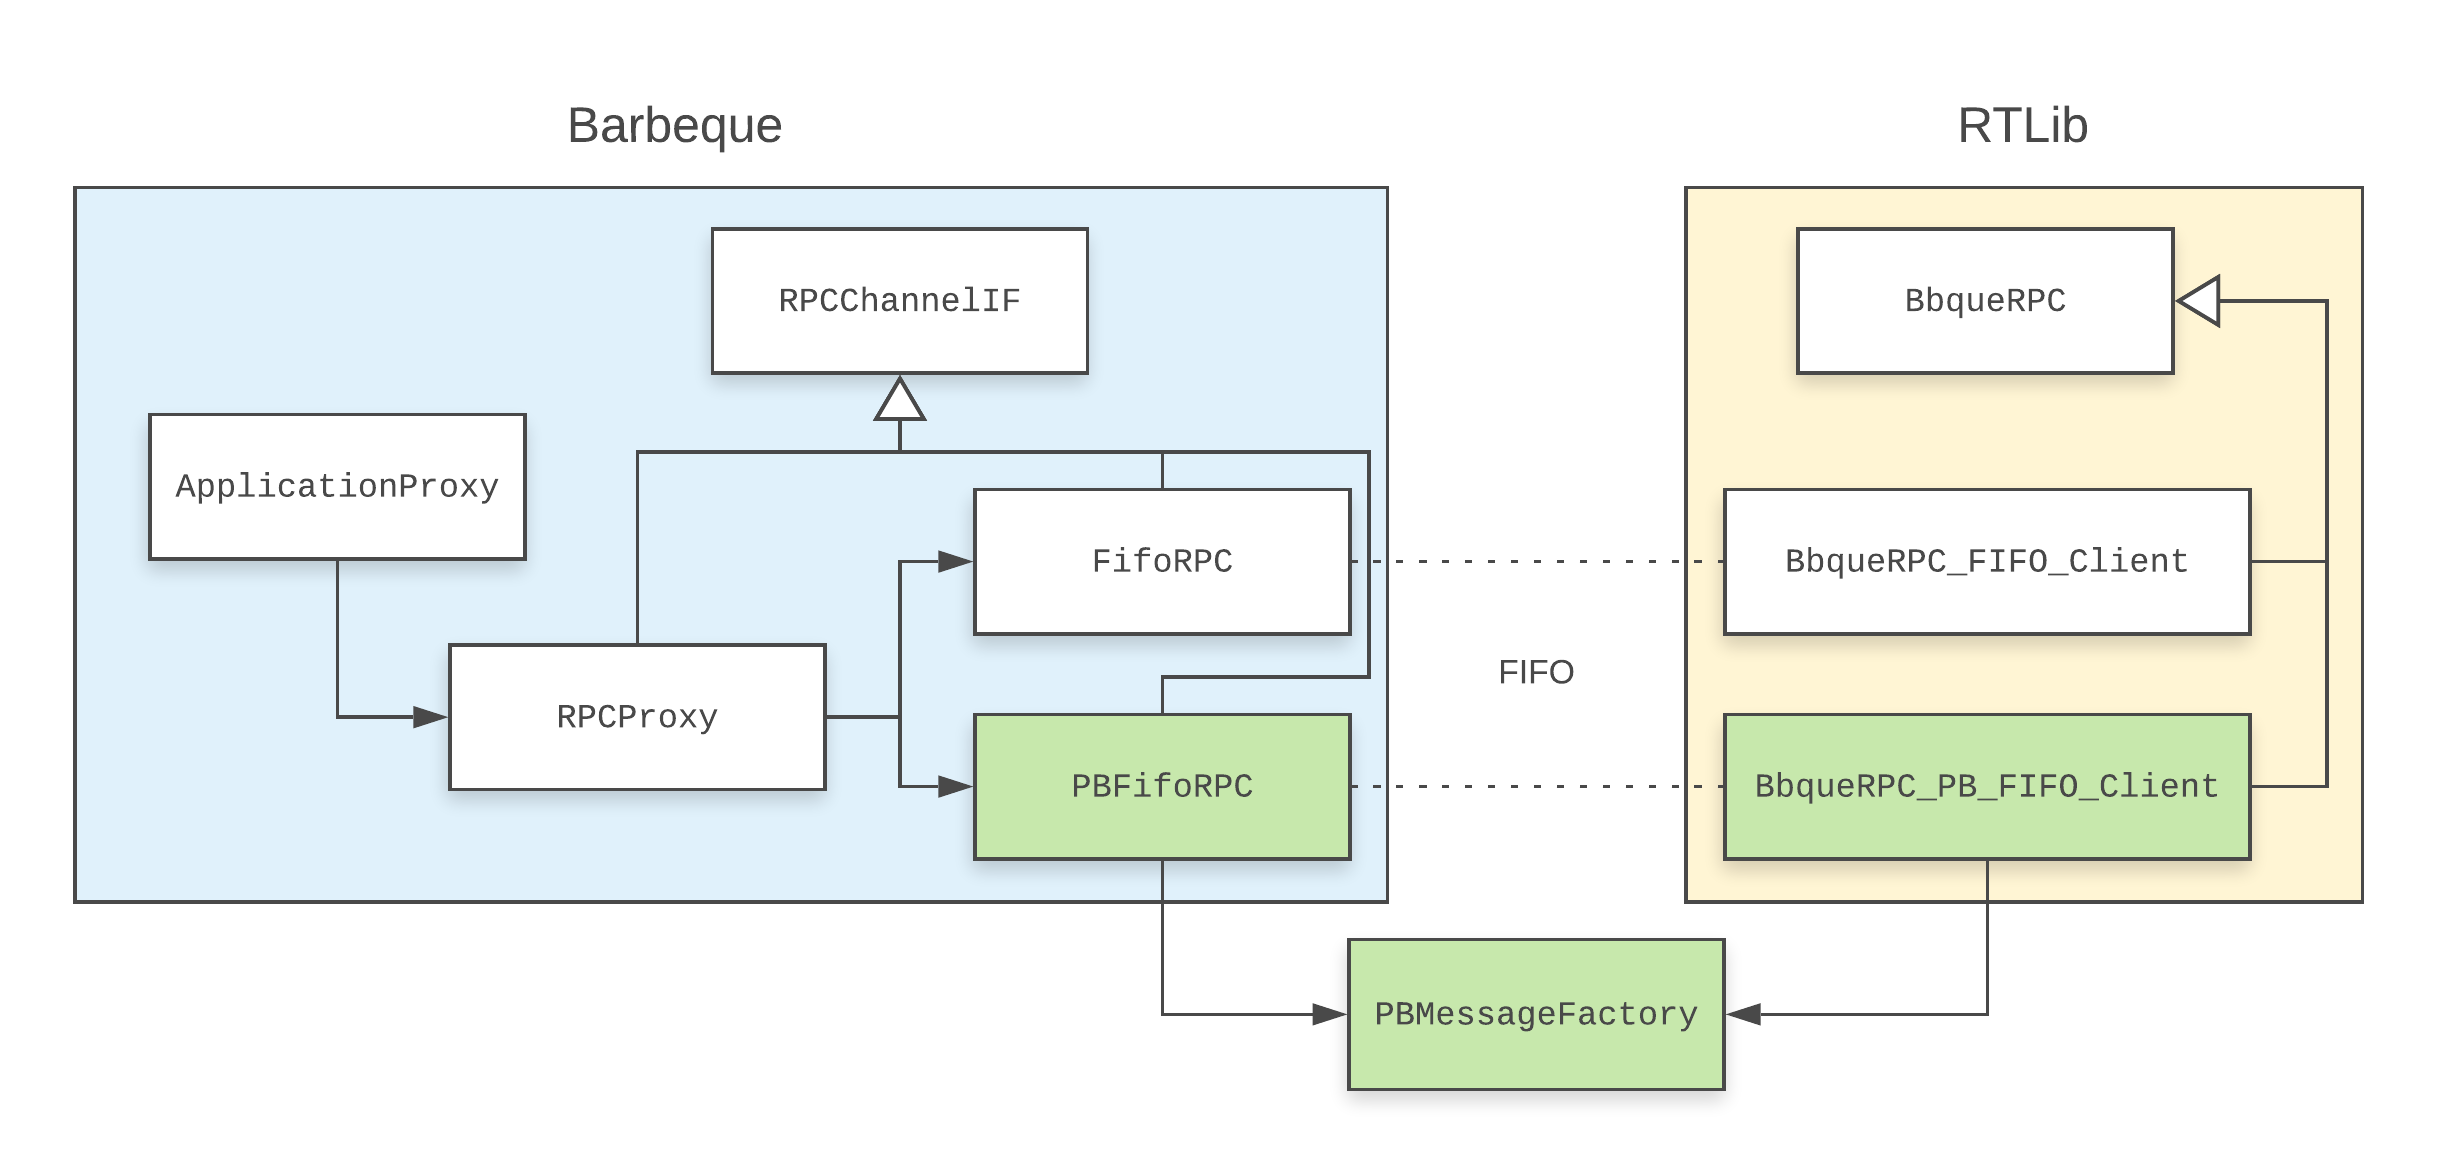
\includegraphics[width=1\linewidth, keepaspectratio]{class-diagram}
    \caption{Class diagram. The classes in green are the new ones.}
    \label{fig:class-diagram}
\end{figure}

\newpage
\section{Experimental evaluation}

The performance evaluation was carried out with the standard UNIX tool \texttt{time}. \prettyref{tab:experiment} contains the experimental values and their average. The slightly higher value of the protobuf average could be purely coincidental or could be due to protobuf data-filling functions requiring more instructions.

\begin{table}[h!]
    \small
    \begin{center}
        \begin{tabular}{|R{1.5cm}|R{1.5cm}|}
            \hline
            \textbf{FIFO} & \textbf{Protobuf} \\ \hline
            \hline
            85 ms & 78 ms \\ \hline
            83 ms & 82 ms \\ \hline
            80 ms & 82 ms \\ \hline
            90 ms & 85 ms \\ \hline
            75 ms & 86 ms \\ \hline
            72 ms & 90 ms \\ \hline
            81 ms & 90 ms \\ \hline
            79 ms & 81 ms \\ \hline
            77 ms & 82 ms \\ \hline
            74 ms & 76 ms \\ \hline
            \hline
            \textbf{80 ms} & \textbf{82 ms} \\ \hline
        \end{tabular}
        \caption{Collection of execution times. The last row contains the average.}
        \label{tab:experiment}
    \end{center}
\end{table}

\section{Conclusions and Future Works}

The current implementation suffers from poorly optimized memory usage: the array used to hold the serialized protobuf data is part of the wrapper \texttt{struct}, and its size is fixed at compile-time. Since such wrapper \texttt{structs} are always declared as local variables, the array is allocated on the stack. The size of the array, 1 KiB, is not a problem for a common x86 machine -- the target platform of this project -- but it could be for an embedded system. For this reason, a smarter approach would be to separate the array from the wrapper struct and to allocate the array on the heap, sizing it so that it exactly fits the serialized data. The actual transmission would be then broken into two parts: first the wrapper \texttt{struct}, then the array.
